\section{Исследовательская часть}

\subsection{Технические характеристики}

Технические характеристики устройства, на котором выполнялся замерный эксперимент:
\begin{itemize}[label*=---]
	\item операционная система macOS  Ventura 13.0.1 \cite{ventura};
	\item память 32 ГБ;
	\item процессор 2,3 ГГц 4-ядерный процессор Intel Core i7.
\end{itemize}

Замеры проводилось на ноутбуке, включенном в сеть электропитания. Во время тестирования ноутбук был нагружен только встроенными приложениями окружения, окружением, а также непосредственно замерным экспериментом.

\subsection{Пример работы программы}

На рисунке \ref{img:example} представлен пример работы программы. Вводится количество кард, далее выводится лог при параллельной обработки и последовательной. 

\begin{figure}[!h]
	\centering
	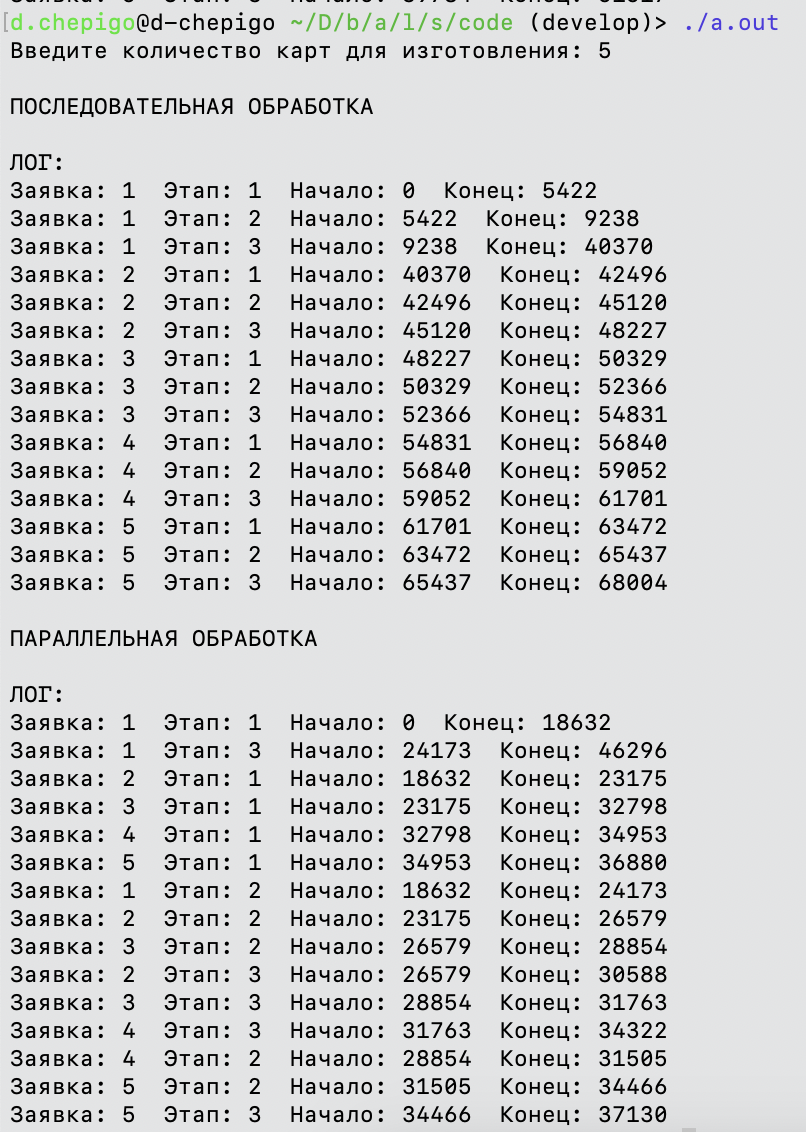
\includegraphics[width=130mm]{images/example}
	\caption{Пример работы программы}
	\label{img:example}
\end{figure}

\pagebreak
\newpage
\subsection{Время выполнения реализованных алгоритмов}
В таблице \ref{tab:time} представлены результаты замера времени реализованных алгоритмов. На рисунке \ref{img:result} представлен график зависимости.
\begin{table}[hbtp]
	\begin{center}
		\begin{flushleft}
			\caption{\label{tab:time}Результаты замеров времени реализованных сортировок в наноосекундах}
		\end{flushleft}
		\begin{tabular}{|l | l | l | l |} 
		\hline {Количество карт} & {Последовательная} & {Параллельная} \\ \hline
		10 & 102686 & 57213   \\ \hline
		20 & 110647   &  60790 \\ \hline
		30 & 126516 & 64714   \\ \hline
		40 &  137995 &  69191 \\ \hline
		50 & 151877 & 91153\\ \hline
		\end{tabular}
	\end{center}
\end{table}

\begin{figure}	\centering
	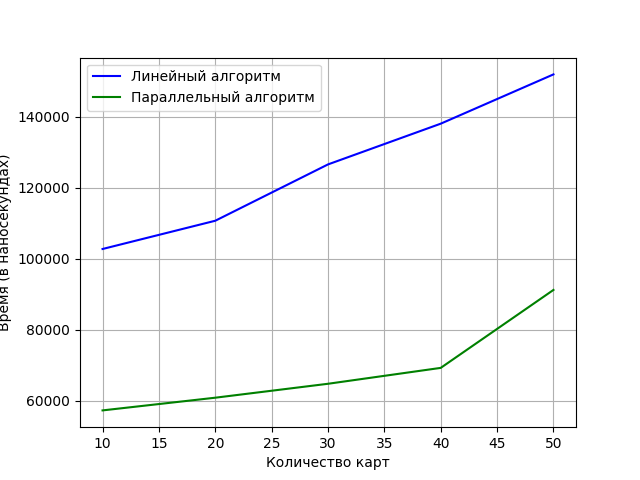
\includegraphics[width=150mm]{images/result}
	\captionsetup{justification=centering}
	\centering\caption{Зависимость времени работы реализованных алгоритмов от количества карт}
	\label{img:result}
\end{figure}
